\documentclass{standalone}
\usepackage{tikz}
\usetikzlibrary{patterns, positioning}


\begin{document}
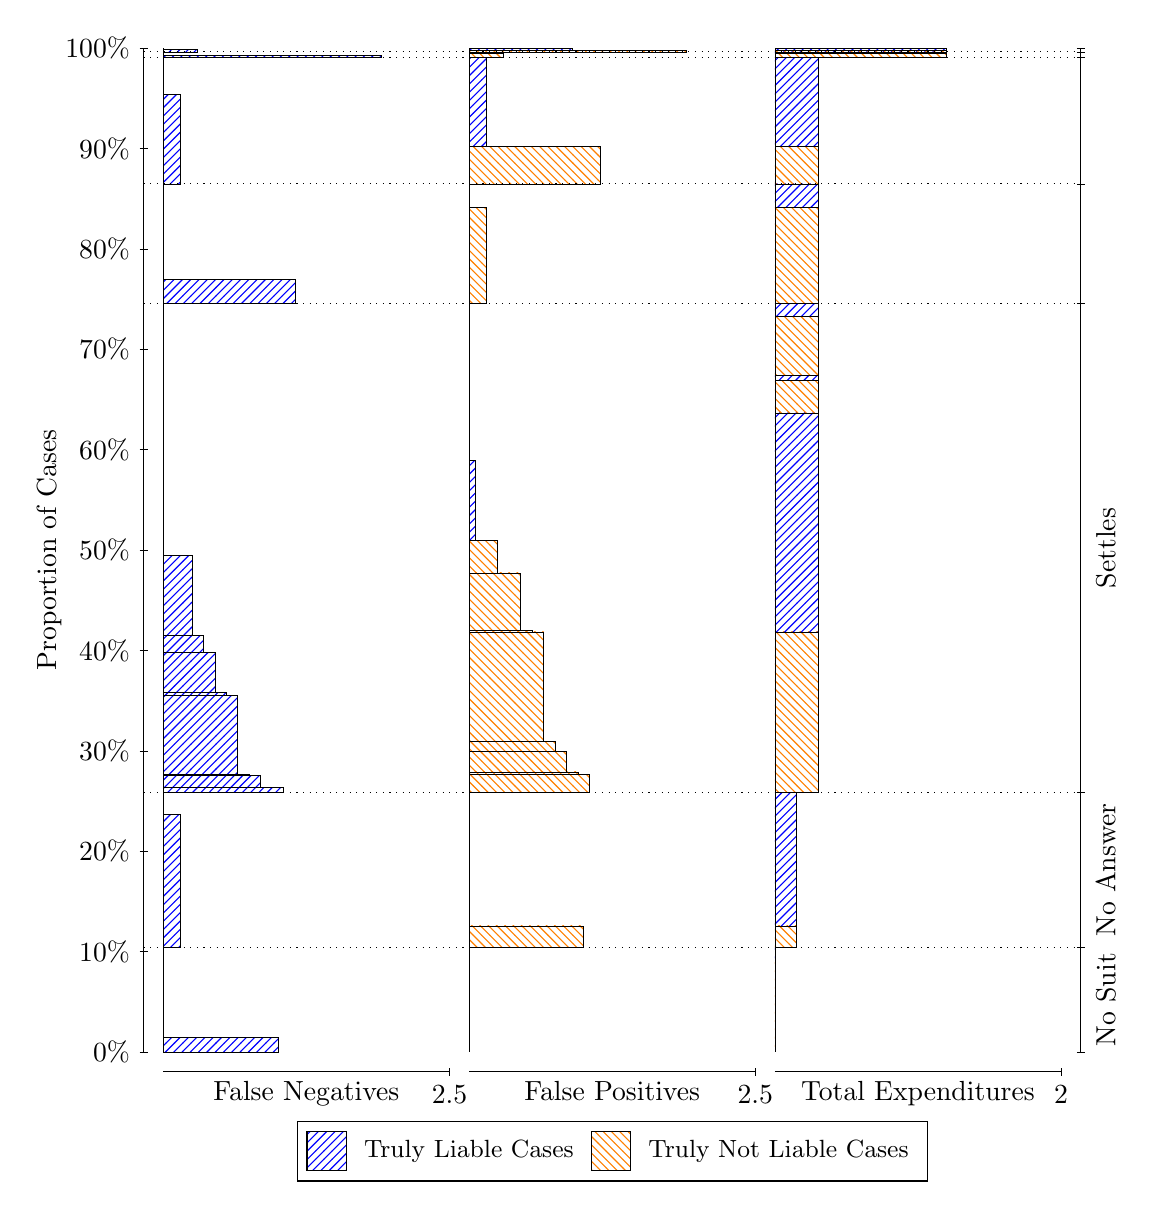
\begin{tikzpicture}
\draw[black, very thin] (1.5,1.75) -- (1.5,14.5);
\node[rotate=90, text=black, anchor=center] at (0.3, 8.125) {Proportion of Cases};
\draw[black, very thin] (1.45,1.75) -- (1.55,1.75);
\node[text=black, anchor=east] at (1.45, 1.75) {0\%};
\draw[black, very thin] (1.45,3.025) -- (1.55,3.025);
\node[text=black, anchor=east] at (1.45, 3.025) {10\%};
\draw[black, very thin] (1.45,4.3) -- (1.55,4.3);
\node[text=black, anchor=east] at (1.45, 4.3) {20\%};
\draw[black, very thin] (1.45,5.575) -- (1.55,5.575);
\node[text=black, anchor=east] at (1.45, 5.575) {30\%};
\draw[black, very thin] (1.45,6.85) -- (1.55,6.85);
\node[text=black, anchor=east] at (1.45, 6.85) {40\%};
\draw[black, very thin] (1.45,8.125) -- (1.55,8.125);
\node[text=black, anchor=east] at (1.45, 8.125) {50\%};
\draw[black, very thin] (1.45,9.4) -- (1.55,9.4);
\node[text=black, anchor=east] at (1.45, 9.4) {60\%};
\draw[black, very thin] (1.45,10.675) -- (1.55,10.675);
\node[text=black, anchor=east] at (1.45, 10.675) {70\%};
\draw[black, very thin] (1.45,11.95) -- (1.55,11.95);
\node[text=black, anchor=east] at (1.45, 11.95) {80\%};
\draw[black, very thin] (1.45,13.225) -- (1.55,13.225);
\node[text=black, anchor=east] at (1.45, 13.225) {90\%};
\draw[black, very thin] (1.45,14.5) -- (1.55,14.5);
\node[text=black, anchor=east] at (1.45, 14.5) {100\%};

\draw[black, very thin] (13.4,1.75) -- (13.4,14.5);
\draw[black, very thin] (13.35,1.75) -- (13.45,1.75);
\node[anchor=west] at (13.35, 1.75) {};
\draw[black, very thin] (13.35,3.0774) -- (13.45,3.0774);
\node[anchor=west] at (13.35, 3.0774) {};
\draw[black, very thin] (13.35,5.0423) -- (13.45,5.0423);
\node[anchor=west] at (13.35, 5.0423) {};
\draw[black, very thin] (13.35,11.255) -- (13.45,11.255);
\node[anchor=west] at (13.35, 11.255) {};
\draw[black, very thin] (13.35,12.776) -- (13.45,12.776);
\node[anchor=west] at (13.35, 12.776) {};
\draw[black, very thin] (13.35,14.384) -- (13.45,14.384);
\node[anchor=west] at (13.35, 14.384) {};
\draw[black, very thin] (13.35,14.451) -- (13.45,14.451);
\node[anchor=west] at (13.35, 14.451) {};
\draw[black, very thin] (13.35,14.5) -- (13.45,14.5);
\node[anchor=west] at (13.35, 14.5) {};

\draw[black, very thin, pattern color=blue, pattern=north east lines] (1.75,1.75) rectangle (3.2033,1.9372);
\draw[black, very thin, pattern color=orange, pattern=north west lines] (1.75,1.9372) rectangle (1.75,3.0774);
\draw[black, very thin, pattern color=blue, pattern=north east lines] (1.75,3.0774) rectangle (1.968,4.7676);
\draw[black, very thin, pattern color=orange, pattern=north west lines] (1.75,4.7676) rectangle (1.75,5.0423);
\draw[black, very thin, pattern color=blue, pattern=north east lines] (1.75,5.0423) rectangle (3.276,5.1122);
\draw[black, very thin, pattern color=blue, pattern=north east lines] (1.75,5.1122) rectangle (2.9853,5.2615);
\draw[black, very thin, pattern color=blue, pattern=north east lines] (1.75,5.2615) rectangle (2.84,5.2732);
\draw[black, very thin, pattern color=blue, pattern=north east lines] (1.75,5.2732) rectangle (2.6947,6.2762);
\draw[black, very thin, pattern color=blue, pattern=north east lines] (1.75,6.2762) rectangle (2.5493,6.3211);
\draw[black, very thin, pattern color=blue, pattern=north east lines] (1.75,6.3211) rectangle (2.404,6.8272);
\draw[black, very thin, pattern color=blue, pattern=north east lines] (1.75,6.8272) rectangle (2.2587,7.0395);
\draw[black, very thin, pattern color=blue, pattern=north east lines] (1.75,7.0395) rectangle (2.1133,8.0549);
\draw[black, very thin, pattern color=orange, pattern=north west lines] (1.75,8.0549) rectangle (1.75,11.255);
\draw[black, very thin, pattern color=blue, pattern=north east lines] (1.75,11.255) rectangle (3.4213,11.557);
\draw[black, very thin, pattern color=orange, pattern=north west lines] (1.75,11.557) rectangle (1.75,12.776);
\draw[black, very thin, pattern color=blue, pattern=north east lines] (1.75,12.776) rectangle (1.968,13.909);
\draw[black, very thin, pattern color=orange, pattern=north west lines] (1.75,13.909) rectangle (1.75,14.384);
\draw[black, very thin, pattern color=blue, pattern=north east lines] (1.75,14.384) rectangle (4.5113,14.402);
\draw[black, very thin, pattern color=orange, pattern=north west lines] (1.75,14.402) rectangle (1.75,14.451);
\draw[black, very thin, pattern color=blue, pattern=north east lines] (1.75,14.451) rectangle (2.186,14.482);
\draw[black, very thin, pattern color=orange, pattern=north west lines] (1.75,14.482) rectangle (1.75,14.5);
\draw[black, very thin, pattern color=orange, pattern=north west lines] (5.6333,1.75) rectangle (5.6333,2.8902);
\draw[black, very thin, pattern color=blue, pattern=north east lines] (5.6333,2.8902) rectangle (5.6333,3.0774);
\draw[black, very thin, pattern color=orange, pattern=north west lines] (5.6333,3.0774) rectangle (7.0867,3.3521);
\draw[black, very thin, pattern color=blue, pattern=north east lines] (5.6333,3.3521) rectangle (5.6333,5.0423);
\draw[black, very thin, pattern color=orange, pattern=north west lines] (5.6333,5.0423) rectangle (7.1593,5.2792);
\draw[black, very thin, pattern color=orange, pattern=north west lines] (5.6333,5.2792) rectangle (7.014,5.3082);
\draw[black, very thin, pattern color=orange, pattern=north west lines] (5.6333,5.3082) rectangle (6.8687,5.5634);
\draw[black, very thin, pattern color=orange, pattern=north west lines] (5.6333,5.5634) rectangle (6.7233,5.6944);
\draw[black, very thin, pattern color=orange, pattern=north west lines] (5.6333,5.6944) rectangle (6.578,7.0852);
\draw[black, very thin, pattern color=orange, pattern=north west lines] (5.6333,7.0852) rectangle (6.4327,7.101);
\draw[black, very thin, pattern color=orange, pattern=north west lines] (5.6333,7.101) rectangle (6.2873,7.8332);
\draw[black, very thin, pattern color=orange, pattern=north west lines] (5.6333,7.8332) rectangle (5.9967,8.243);
\draw[black, very thin, pattern color=blue, pattern=north east lines] (5.6333,8.243) rectangle (5.706,9.2583);
\draw[black, very thin, pattern color=blue, pattern=north east lines] (5.6333,9.2583) rectangle (5.6333,11.255);
\draw[black, very thin, pattern color=orange, pattern=north west lines] (5.6333,11.255) rectangle (5.8513,12.474);
\draw[black, very thin, pattern color=blue, pattern=north east lines] (5.6333,12.474) rectangle (5.6333,12.776);
\draw[black, very thin, pattern color=orange, pattern=north west lines] (5.6333,12.776) rectangle (7.3047,13.251);
\draw[black, very thin, pattern color=blue, pattern=north east lines] (5.6333,13.251) rectangle (5.8513,14.384);
\draw[black, very thin, pattern color=orange, pattern=north west lines] (5.6333,14.384) rectangle (6.0693,14.433);
\draw[black, very thin, pattern color=blue, pattern=north east lines] (5.6333,14.433) rectangle (5.6333,14.451);
\draw[black, very thin, pattern color=orange, pattern=north west lines] (5.6333,14.451) rectangle (8.3947,14.468);
\draw[black, very thin, pattern color=blue, pattern=north east lines] (5.6333,14.468) rectangle (6.9413,14.5);
\draw[black, very thin, pattern color=orange, pattern=north west lines] (9.5167,1.75) rectangle (9.5167,2.8902);
\draw[black, very thin, pattern color=blue, pattern=north east lines] (9.5167,2.8902) rectangle (9.5167,3.0774);
\draw[black, very thin, pattern color=orange, pattern=north west lines] (9.5167,3.0774) rectangle (9.7892,3.3521);
\draw[black, very thin, pattern color=blue, pattern=north east lines] (9.5167,3.3521) rectangle (9.7892,5.0423);
\draw[black, very thin, pattern color=orange, pattern=north west lines] (9.5167,5.0423) rectangle (10.062,7.0852);
\draw[black, very thin, pattern color=blue, pattern=north east lines] (9.5167,7.0852) rectangle (10.062,9.8668);
\draw[black, very thin, pattern color=orange, pattern=north west lines] (9.5167,9.8668) rectangle (10.062,10.277);
\draw[black, very thin, pattern color=blue, pattern=north east lines] (9.5167,10.277) rectangle (10.062,10.346);
\draw[black, very thin, pattern color=orange, pattern=north west lines] (9.5167,10.346) rectangle (10.062,11.094);
\draw[black, very thin, pattern color=blue, pattern=north east lines] (9.5167,11.094) rectangle (10.062,11.255);
\draw[black, very thin, pattern color=orange, pattern=north west lines] (9.5167,11.255) rectangle (10.062,12.474);
\draw[black, very thin, pattern color=blue, pattern=north east lines] (9.5167,12.474) rectangle (10.062,12.776);
\draw[black, very thin, pattern color=orange, pattern=north west lines] (9.5167,12.776) rectangle (10.062,13.251);
\draw[black, very thin, pattern color=blue, pattern=north east lines] (9.5167,13.251) rectangle (10.062,14.384);
\draw[black, very thin, pattern color=orange, pattern=north west lines] (9.5167,14.384) rectangle (11.697,14.433);
\draw[black, very thin, pattern color=blue, pattern=north east lines] (9.5167,14.433) rectangle (11.697,14.451);
\draw[black, very thin, pattern color=orange, pattern=north west lines] (9.5167,14.451) rectangle (11.697,14.468);
\draw[black, very thin, pattern color=blue, pattern=north east lines] (9.5167,14.468) rectangle (11.697,14.5);
\draw[black, dotted] (1.5,3.0774) -- (13.4,3.0774);
\draw[black, dotted] (1.5,5.0423) -- (13.4,5.0423);
\draw[black, dotted] (1.5,11.255) -- (13.4,11.255);
\draw[black, dotted] (1.5,12.776) -- (13.4,12.776);
\draw[black, dotted] (1.5,14.384) -- (13.4,14.384);
\draw[black, dotted] (1.5,14.451) -- (13.4,14.451);
\draw[black, very thin] (1.75,1.5) -- (5.3833,1.5);
\node[text=black, anchor=north] at (3.5667, 1.5) {False Negatives};
\draw[black, very thin] (5.3833,1.45) -- (5.3833,1.55);
\node[text=black, anchor=north] at (5.3833, 1.45) {2.5};

\draw[black, very thin] (5.6333,1.5) -- (9.2667,1.5);
\node[text=black, anchor=north] at (7.45, 1.5) {False Positives};
\draw[black, very thin] (9.2667,1.45) -- (9.2667,1.55);
\node[text=black, anchor=north] at (9.2667, 1.45) {2.5};

\draw[black, very thin] (9.5167,1.5) -- (13.15,1.5);
\node[text=black, anchor=north] at (11.333, 1.5) {Total Expenditures};
\draw[black, very thin] (13.15,1.45) -- (13.15,1.55);
\node[text=black, anchor=north] at (13.15, 1.45) {2};

\node[text=black, centered, rotate=90] at (13.72, 2.4137) {No Suit};
\node[text=black, centered, rotate=90] at (13.72, 4.0599) {No Answer};
\node[text=black, centered, rotate=90] at (13.72, 8.1489) {Settles};





\draw (7.449999999999999,1.5) node[draw=none] (baseCoordinate) {};
\begin{scope}[align=center]
        \matrix[scale=0.5, draw=black, below=0.5cm of baseCoordinate, nodes={draw}, column sep=0.1cm]{
            \node[rectangle, draw, minimum width=0.5cm, minimum height=0.5cm, pattern color=blue, pattern=north east lines] {}; &
            \node[draw=none, font=\small, text=black] (B) {Truly Liable Cases}; &
            \node[rectangle, draw, minimum width=0.5cm, minimum height=0.5cm, pattern color=orange, pattern=north west lines] {}; &
            \node[draw=none, font=\small, text=black] (B) {Truly Not Liable Cases}; \\
            };
\end{scope}

\end{tikzpicture}
\end{document}